\chapter[Analysis]{Analysis}\label{chap:analysis}

This chapter constitutes the core of this dissertation. Here, we will discuss the analysis conducted, starting with a general overview, followed by an explanation of the samples, triggers, and object definitions. We will then talk about the corrections applied to the data and simulations to enhance the analysis results. Additionally, we will cover the criteria used in event selection and how the signal and background have been modeled. Finally, we will present the expected upper limits of the branching ratio for each channel, as this analysis will only be working with simulated signal, alongside simulated and real background data. The chapter concludes by addressing the subsequent steps required before data unblinding and the attainment of the final experimental measurement, as well as suggesting other ideas to improve the results.

\section{Analysis overview}\label{sec:analysis_overview}

This analysis uses data from proton-proton collisions corresponding to an integrated luminosity of 39.54 fb$^{-1}$ at $\sqrt{s}=$13 TeV, collected by the CMS detector at LHC in 2018 during Run 2. It only targets the Higgs boson production mode via gluon fusion (ggH), which accounts for approximately 87\% of the Higgs boson production at LHC at $\sqrt{s}=$13 TeV. Although it is possible to extend this analysis to include more production modes, time constraints have led us to focus to the main production channel. The final states of interest consist of an isolated and energetic photon, a charged meson pair, and photons compatible with a third (and sometimes fourth) neutral meson, with 0 hadronic jets and no additional leptons ($e/\mu$). The mesons considered here are a $\phi$, a $\omega$ and a $D^{*0}$, each further decaying into two charged particles and a third (and fourth) neutral one (see Table \ref{tab:Higgs_rare_decays_three}).

\begin{table}[ht]
    \centering
    \begin{tabular}{ll}
        $\text{H}\decaysto \phi\gamma$ ,& $\phi\decaysto \pi^+\pi^-\pi^0$ \\
        $\text{H}\decaysto \omega\gamma$ ,& $\omega\decaysto \pi^+\pi^-\pi^0$\\
        $\text{H}\decaysto D^{*0}\gamma$ ,& $D^{*0}\decaysto D^{0}\pi^{0}/\gamma,\ D^{0}\decaysto K^{\mp}\pi^{\pm}$\\
        $\text{H}\decaysto D^{*0}\gamma$ ,& $D^{*0}\decaysto D^{0}\pi^{0}/\gamma,\ D^{0}\decaysto K^{\mp}\pi^{\pm}\pi^{0}$
    \end{tabular}
    \caption{Higgs rare decays under study in this analysis.}
    \label{tab:Higgs_rare_decays_three}
\end{table}

The analysis strategy involves categorizing events to increase the signal to background ratio. In our production mode (ggH), the largest background source in this analysis consists of $\gamma$ plus jets events.

The branching fractions of rare Higgs boson decays to a meson and photon can be computed using a factorization approach in QCD. The calculation considers both direct and indirect contributions, as explained in the first chapter and depicted in Figure \ref{fig:Higgs_rare_decay_veritces}. The interference between these components is significant. In the SM, the indirect component dominates, and the Higgs boson couplings to light quarks are probed by searching for modifications in this branching fraction due to interference effects.

As previously explained, given the exotic nature of the decays under study, the theoretical decay widths being so small, the large hadronic background at the LHC, and the limited amount of data collected, we cannot aim for precise measurements of the branching fractions. Instead, the end goal of this thesis is to calculate a reasonable upper limit on the branching ratio of the aforementioned Higgs boson decays, using Monte Carlo (MC) samples to model the SM expected signal. To obtain a competitive, real result, this initial estimation requires further refinement and improvement, such as considering additional background sources, systematic uncertainties, etc.

The main difference between this analysis and the study of the three decays in the upper half of Table \ref{tab:Higgs_rare_decays} is that, in contrast to those, we are studying 3-body decays with neutral particles, which are more challenging to track than charged ones. The framework used for this analysis builds upon the existing framework for the simpler two-body decays currently under analysis by the Particle Physics Collaboration at MIT. To extend their study to include three-body decays involving neutral particles, our main focus has been on accurately recovering the missing neutral particles.

\section{Samples and triggers}\label{sec:samples_triggers}

To develop this analysis, the data file format used is one designed by CMS, which is an extended version of \verb+NANOAOD+. It is based on the official \verb+NANOAODv9+ recipe and includes the reconstructed mesons, as described in Section \ref{sec:objects}, as additional objects. The \verb+NANOAOD+ format consists of an Ntuple-like structure used by CMS, which can be read using bare root, and containing the per-event information that is needed in most generic analyses \cite{CMS:NanoAOD}. This analysis is performed using the \verb+ROOT+ data analysis framework, an open-source data analysis tool commonly used in high energy physics written mainly in C++ \cite{CERN:root}.

\subsection{Data and Tau trigger}

Events are selected from proton-proton collision data at a center-of-mass energy of $\sqrt{s}=$13 TeV and a bunch spacing of 25 ns, collected by the CMS experiment during the LHC's Run 2 in 2018, corresponding to a total integrated luminosity of 39.54 fb$^{-1}$. Good run ranges and luminosity blocks are chosen based on criteria encoded in a golden JSON file.

To filter data in the gluon fusion production mode, a tau-like trigger is employed. This Tau trigger selects a photon with $\pT^{\gamma} > 35\ \GeV$ and a ditrack system with $\pT^{\text{jet}} > 35\ \GeV$, after going through the L1 trigger, which also imposes rapidity restrictions of $\abs{\eta^{\gamma}}<2.1$ and $\abs{\eta^{\text{jet}}}<2.1$. The trigger is applied to both data and MC. Introduced in 2018, this trigger recorded events enriched in gluon fusion production of the Higgs boson and VBF that were not registered by the dedicated trigger, providing an effective luminosity of 39.54 fb$^{-1}$. The trigger selecting events during 2018 is encoded as \verb+Photon35_TwoProngs35+. \todo{Should I include trigger efficiencies for each channel in the appendix? If so, how do I obtain these plots?} The datasets used in gluon fusion and VBF analysis are detailed in Table \ref{tab:ggH_datasets}.

\begin{table}[ht]
    \centering
    \begin{tabular}{|c|c|c|}
        \hline
        \multicolumn{1}{|c|}{\cellcolor{lightgray}Year} & \cellcolor{lightgray}Dataset & \cellcolor{lightgray}Integrated luminosity [fb$^{-1}$] \\ \hline
        2018    & \verb+/Tau/Run2018B-UL2018+  & 0.67 \\
        2018    & \verb+/Tau/Run2018C-UL2018+  & 6.94 \\
        2018    & \verb+/Tau/Run2018D-UL2018+  & 31.93 \\ \hline
    \end{tabular}
    \caption{Datasets used in the gluon fusion analysis from the campaign MiniAODv2 of the MINIAOD data tier.}
    \label{tab:ggH_datasets}
\end{table}

\subsection{Background simulation}

The background estimation will ultimately rely solely on data. However, at the early stage of this analysis, simulated samples are used to understand the background processes affecting the different selected final states. The main background process for the gluon fusion production mode is a single photon and jets.

Every event is generated at leading order (LO) precision using the MADGRAPH5 generator \verb+MG5_aMC@NLO+ \cite{Alwall:2014hca} and POWHEG \cite{Alioli:2010xd}, while PYTHIA8 \cite{Sjostrand:2014zea} is used for the hadronization. For all simulations, the NNPDF 3.1 \cite{NNPDF:2017mvq} next-to-next-to-leading-order (NNLO) parton distribution functions (PDFs) are used, while the modeling of the underlying event is generated using the CMS Pythia 5 (CP5) tunes \cite{CMS:2019csb}. The Run 2 legacy reconstruction algorithms \cite{Elmetenawee:2020emw} are used for all the MC and data samples. The campaign and global tag used to produce the background and signal MC samples are \verb+RunIISummer20UL18MiniAODv2-106X+ and \verb+upgrade2018_realistic_v16_L1v1+, respectively. Table \ref{tab:MC_samples} summarizes the list of datasets used for the study along with their cross sections \cite{CERN:xsdb}.

\begin{table}[ht]
    \centering
    \begin{tabular}{|l|c|}
        \hline
        \multicolumn{1}{|c|}{\cellcolor{lightgray}Monte Carlo name} & \cellcolor{lightgray}Cross section [pb] \\ \hline
        \verb+GJets_HT-40To100_TuneCP5_13TeV-madgraphMLM-pythia8+  & 18540 (LO) $\times$ 1.26 \\
        \verb+GJets_HT-100To200_TuneCP5_13TeV-madgraphMLM-pythia8+  & 8644 (LO) $\times$ 1.26 \\
        \verb+GJets_HT-200To400_TuneCP5_13TeV-madgraphMLM-pythia8+  & 2183 (LO) $\times$ 1.26 \\
        \verb+GJets_HT-400To600_TuneCP5_13TeV-madgraphMLM-pythia8+  & 260.2 (LO) $\times$ 1.26 \\
        \verb+GJets_HT-600ToInf_TuneCP5_13TeV-madgraphMLM-pythia8+  & 86.58 (LO) $\times$ 1.26 \\ \hline
    \end{tabular}
    \caption{MC samples used for the gluon fusion production mode. The normalization of $\gamma+$jets is scaled by 1.26 \cite{CMS:2018qao} \todo{WHY?}.}
    \label{tab:MC_samples}
\end{table}

\subsection{Signal simulation}

The only Higgs boson production mode studied, gluon fusion, is generated at next-to-leading order (NLO) using the POWHEGv2 event generator extended with the MiNLO procedure \cite{Hamilton:2012np}. The production rates and kinematic distributions for the Higgs boson with $m_H=125\ \GeV$ are assumed throughout. In particular, the cross section for gluon fusion is computed at NNLO in QCD and NLO in electroweak accuracy, resulting in 48.58 pb, as provided by the LHC Higgs Cross Section Working Group in Ref. \cite{LHCHiggsCrossSectionWorkingGroup:2016ypw}.

The decay of the Higgs boson is handled by Pythia. Direct and indirect effective vertices are not simulated. The expected SM branching fractions of the Higgs rare decays are as previously shown in Table \ref{tab:Higgs_rare_decays_values}: $\mathcal{B}(\text{H}\decaysto \phi\gamma) = (2.31 \pm 0.11)\times 10^{-6}$ and $\mathcal{B}(\text{H}\decaysto \omega\gamma) = (1.48 \pm 0.08)\times 10^{-6}$, while $\mathcal{B}(\text{H}\decaysto D^{*0}\gamma)$ has not yet been computed. In the analysis, however, the branching ratios are set to
\begin{equation*}
    \mathcal{B}(\text{H}\decaysto \phi\gamma) = \mathcal{B}(\text{H}\decaysto \omega\gamma) = \mathcal{B}(\text{H}\decaysto D^{*0}\gamma) = 1\ ,
\end{equation*}
because \todo{explain why}. The branching fractions of the meson decays used are also shown in Table \ref{tab:Higgs_rare_decays}, but further detailed in Table \ref{tab:Meson_decay_br}.

\begin{table}[!ht]
    \centering
    \begin{tabular}{|l|c|}
        \hline
        \multicolumn{1}{|c|}{\cellcolor{lightgray}Meson decay channel} & \multicolumn{1}{c|}{\cellcolor{lightgray} SM $\mathcal{B}$ (\%)} \\ \hline
        $\phi\decaysto \pi^+\pi^-\pi^0$     & $15.4 \pm 0.4$   \\
        $\omega\decaysto \pi^+\pi^-\pi^0$   & $89.2 \pm 0.7$   \\
        $D^{*0}\decaysto D^{0}\pi^0$        & $64.7 \pm 0.9$   \\
        $D^{*0}\decaysto D^{0}\gamma$       & $35.3 \pm 0.9$   \\
        $D^{0}\decaysto K^{\mp}\pi^{\pm}$           & $3.962 \pm 0.031$   \\
        $D^{0}\decaysto K^{\mp}\pi^{\pm}\pi^0$      & $14.43 \pm 0.50$   \\
        \hline
    \end{tabular}
    \caption{Meson decay branching ratios used throughout the analysis, from the PDG \cite{PDG}.}
    \label{tab:Meson_decay_br}
\end{table}

\section{Object definitions}\label{sec:objects}

This analysis primarily relies on photons and charged tracks to extract the final state signature of exclusive hadronic decays, while also making use of other physics objects such as additional leptons (or the lack thereof) and hadronic jets to suppress background. All used objects, except the mesons, are discussed in this section, with the next section dedicated solely to meson reconstruction.
\vspace*{-6pt}
\begin{myitemlist}
    \item[Primary vertex (PV):] To consider an event, it must contain at least one primary vertex, which is regarded as the vertex of the hard interaction. There should be a minimum of four tracks associated with the selected primary vertex (from the Higgs boson, the photon and the ditrack system). For events with multiple selected vertices, the PV is chosen to be the vertex corresponding to the hardest scattering in the event, determined using tracking information alone, as described in Ref. \cite{Contardo:2015bmq}.

    \item[Jets:] During the reconstruction of a proton-proton (pp) collision, jets are often reconstructed with a $\pT$ that differs from that of the final-state particles within the jet. The jet energy corrections (JEC) adjust the reconstructed jet energy to match the true energy of the final-state particles. The CMS collaboration has developed a factorized approach to these JEC, consisting of multiple levels that correct various physics or detector effects. This approach provides flexibility in the corrections to suit various types of analyses. These correction levels are commonly referred to as L1FastJet, L2Relative, L3Absolute, and L2L3Residual.

    The flow of these JEC is as follows: Jets are reconstructed from particle flow (PF) candidates using the anti-$k_\text{T}$ clustering algorithm with a distance parameter of $R = 0.4$ as implemented by FastJet \cite{Cacciari:2011ma}. Jets within this small cone (referred to as AK4 jets for $R = 0.4$) are selected among those with $\pT > 25\ \GeV$ and $\abs{\eta} < 4.7$ for forward tagging. At the LHC, a significant number of pp collisions occur simultaniously during one bunch crossing, with soft ones contaminating the collision of interest. To mitigate this effect, known as \textit{pileup} (PU), charged hadrons not originating from the primary vertex are removed using the charged hadron subtraction (CHS) algorithm \cite{CMS:2014ata, Perloff:2012wpa}. The tight pileup ID criterion is applied to reduce the contamination of jets with $\pT < 50\ \GeV$ initiated by the pileup interactions. Jets are corrected for the response inside the detector, differentially in $\abs{\eta} - \abs{\phi}$, for the pileup contributions, and for data only, the residual difference observed between data and simulation.
    
    In the current analysis version, the \verb+Summer19UL+ jet energy corrections set is used, as well as the DeepJet tagging algorithm with the medium working point to identify $b$-jets \cite{Bols:2020bkb}.

    \item[Missing energy:] The $\pT^{\text{miss}}$ measures the transverse momentum imbalance in the event. To estimate it, the deepMET algorithm \cite{Feng:2744871} is used, and $\pT^{\text{miss}}$ filters are then applied to account for instrumental noise in the detector and minimize the impact of the non-collisional background.
    
    \item[Photons:] Photon candidates are reconstructed as SuperCluster objects in the ECAL with $\ET > 38\ \GeV$ and $\abs{\eta^{\gamma}} < 2.1$ in both the barrel and endcap regions. In addition, photons have to satisfy the multivariate analysis (MVA) based selection identification (mvaID) criteria following the \verb+Fall17IsoV2+ recipe \cite{CMS:2020uim}. For the production mode used, the mvaID provides 80\% (90\%) signal selection efficiency for the endcap (barrel) region. The mvaID criteria include photon isolation, charged hadron isolation, and require photons to pass shower shape preselection cuts \cite{Rembser:2019ijh}. The photon's ECAL cluster must be inconsistent with charged particle tracks reconstructed in the silicon tracker to reject electrons faking photons, achieved using a conversion safe electron veto. Residual $\ET$ -dependent photon energy scale and smearing corrections are applied. Additional photons with looser requirements ($\ET > 20\ \GeV$ and the WP90 version of the photonID) are also vetoed to reduce the potential contribution of diphotons. Table \ref{tab:photon_selection} summarizes the criteria for photon selection.

    \begin{table}[!ht]
        \centering
        \begin{tabular}{|l|c|}
            \hline
                \multicolumn{2}{|c|}{\cellcolor{lightgray}Selection criteria ($\gamma$ from PV)}\\ \hline
                $\pT^{\gamma}$            &$>38$ GeV\\
                $\abs{\eta^{\gamma}}$       &$<2.1$ \\
                mvaID                       &WP90/WP80 \\
                electron Veto               &Yes \\\hline
            \end{tabular}
        \caption{Selection criteria applied to the photon from the primary vertex.}
        \label{tab:photon_selection}
    \end{table}
\end{myitemlist}

\section{Meson reconstruction \todo{ADD FOURTH D0* CHANNEL}}\label{sec:meson_reconstruction}

The $\phi$, $\omega$ and $D^{*0}$ mesons decay products are reconstructed using charged particle tracks measured in the tracker, as well as energy deposited in the ECAL compatible with neutral particles coming also from the PV. For the $\phi$ and $\omega$ mesons, the targeted charged ditrack is $\pi^\pm\pi^\mp$, while for the $D^{*0}$ meson the charged ditrack is $K^{\mp}\pi^{\pm}$.

In the following sections, the term \textit{ditrack system} will refer to the system of the two charged tracks, and even though they not form a real particle, notions like ditrack mass will be used (understand the mass of the ditrack as the mass component of the sum of the four-momenta of both tracks). To refer to the meson originating from the PV, namely $\phi$, $\omega$ and $D^{*0}$, terms like \textit{meson} or \textit{full meson} will be used, emphasizing that the neutral particles have been accounted for. Some considerations have been made to precisely reconstruct the full meson:
\vspace*{-6pt}
\begin{myitemlist}
    \item[Track selection:] To be selected, the tracks need to satisfy a ``high purity'' reconstruction criteria, which considers the number of tracker layers with hits, track fit quality, and the impact parameter values relative to their uncertainties. For a detailed description of the algorithm, refer to Ref. \cite{CMS:2014pgm}.

    \item[Meson decay vertex:] The meson decay vertex is determined using the standard CMSSW \cite{CMSSW} kinematic vertex fitting package, as described in Ref. \cite{Prokofiev:2005zz}. Using the candidate's decay vertex and its associated momentum, a newly fitted transient track is constructed to represent the meson candidate. Then, for each primary vertex, the track is extrapolated to the nearest point in 3D space. The meson vertex's longitudinal distance is required to be within 24 cm from the center of the detector.
    
    \item[Isolation:] To ensure good track selection, a dedicated isolation criterion of the candidate based on the tracks is used. This dimensionless isolation parameter (Iso) is determined from the meson's momentum and other tracks within a cone of radius $\Delta R = 0.3$ around the ditrack system's direction. Only tracks with $\pT > 0.9\ \GeV$ associated with the same meson vertex are considered, excluding the charged-hadron candidates that define the ditrack. The definition is as follows:
    \begin{equation*}
        \text{Iso} = \frac{\pT^{\text{meson}}}{\pT^{\text{meson}}+\sum_{\text{trk}}{\abs{\pT^{\text{trk}}}}}
    \end{equation*}
    A high isolation value will be required to consider a meson candidate (over 0.9).

    \item[Neutral particle photons:] For each selected ditrack, up to two photons with $\pT > 5 \ \GeV$ are recovered in a small cone of $\Delta R = 0.05$ around the ditrack direction. These photons account for the recovery of neutral particles, as $\pi^{0}\decaysto\gamma\gamma$ in $\sim 98.8\%$ \cite{PDG}. From generation-level MC we know that photons coming from neutral particle decays that in turn come from the three-body decays must be very collimated with the ditrack system. In the case of the $\phi$/$\omega$ channels and the $D^{*0}$ channel when $D^{0}$ decays into three bodies, these photons directly originate from the $\pi^0$ of the three-body decay. In the case of the $D^{*0}$ channel, the photon comes either directly from $D^{*0}\decaysto D^{0}\gamma$ or from de decay of the $\pi^0$ from $D^{*0}\decaysto D^{0}\pi^0$.
    
    \item[Ditrack mass hypothesis:] The invariant mass of the refitted ditrack system is also used to reduce contamination from background events. The mass of the pair, assuming the charged-pion hypothesis for the two tracks, is consistent with the charged components of the $\phi$ and $\omega$ mesons. Since the ditrack system is not a real resonance, its mass is very wide but consistent and useful for reducing background events. In the case of the $D^{*0}$ channel, two scenarios are considered. On the one hand, when $D^{0}$ decays into a pair of charged particles (kaon-pion) the ditrack system's invariant mass is a real narrow resonance (namely $D^{0}$) coherent with the mass of that meson. On the other hand, when $D^{0}$ decays into a pair of charged particles and a neutral pion, one finds the same scenario as for the $\phi$/$\omega$ decay channels.
    
    The exact used selection criteria will be presented at the end of this section, but it is worth noting that for the $\phi$/$\omega$ three-body decays involving a $\pi^0$, the mass of the ditrack is approximately two-thirds of the full meson's mass (each pion carries roughly a third of the energy).

    Furthermore, instead of recovering the ditrack invariant mass by only retrieving the mass component of the sum of both four-momenta, the CMSSW kinematic fit has been employed. To study the performance of this fit, it is useful to define the \textit{residual} as the difference between the reconstructed values and the corresponding generation-level ones. Figure \ref{fig:kinematic_fit_residuals} displays the residual of the ditrack invariant mass reconstruction with and without the kinematic fits with vertex constraint for every decay mode.
    \begin{figure}[!ht]
        \captionsetup[subfigure]{labelformat=empty}
        \vspace*{-0.2cm}
        \centering
        \setlength{\mylength}{\textwidth}
        \begin{subfigure}[t]{0.50\mylength}
                \centering
                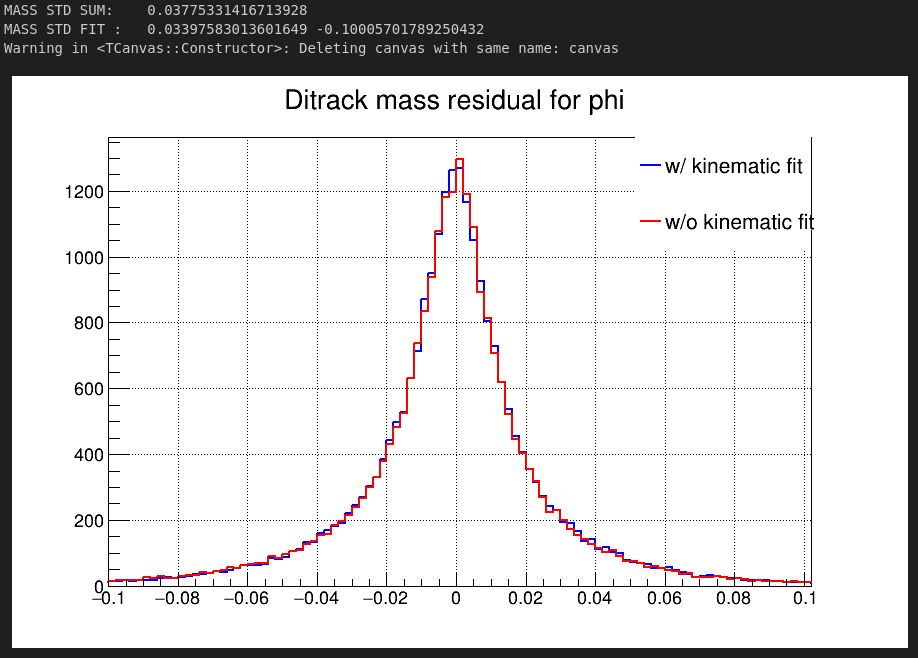
\includegraphics[width=0.45\mylength]{resources/plots/kinematic_fit_residual_phi.png}
                \caption{\footnotesize (a)}
        \end{subfigure}%
        \begin{subfigure}[t]{0.50\mylength}
                \centering
                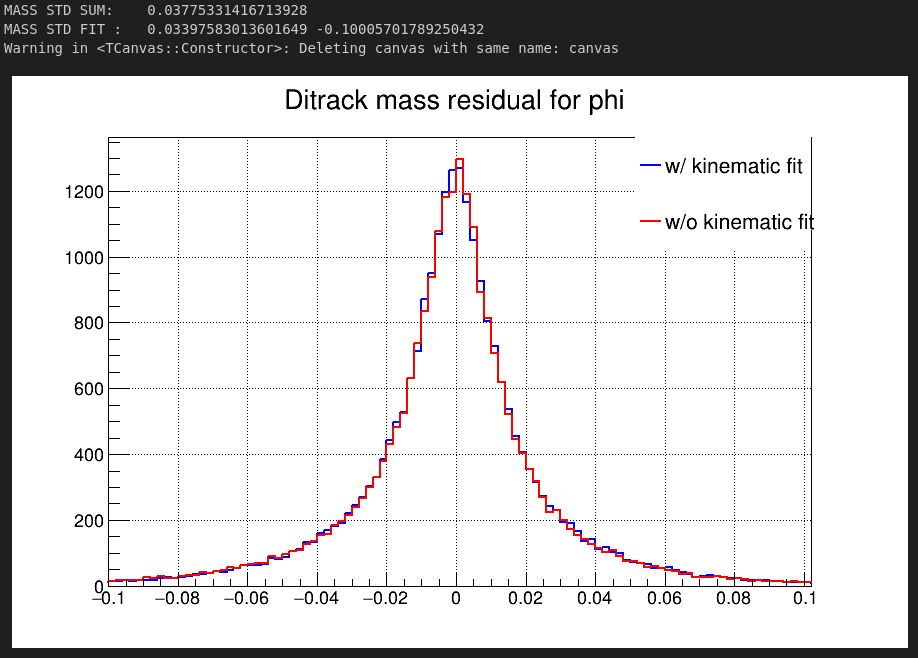
\includegraphics[width=0.45\mylength]{resources/plots/kinematic_fit_residual_omega.png}
                \caption{\footnotesize (b)}
        \end{subfigure}%\begin{subfigure}[t]{0.50\mylength}\baselineskip    
        \vskip\baselineskip
        \vspace*{-0.1cm}
        \begin{subfigure}[t]{0.50\mylength}
                \centering
                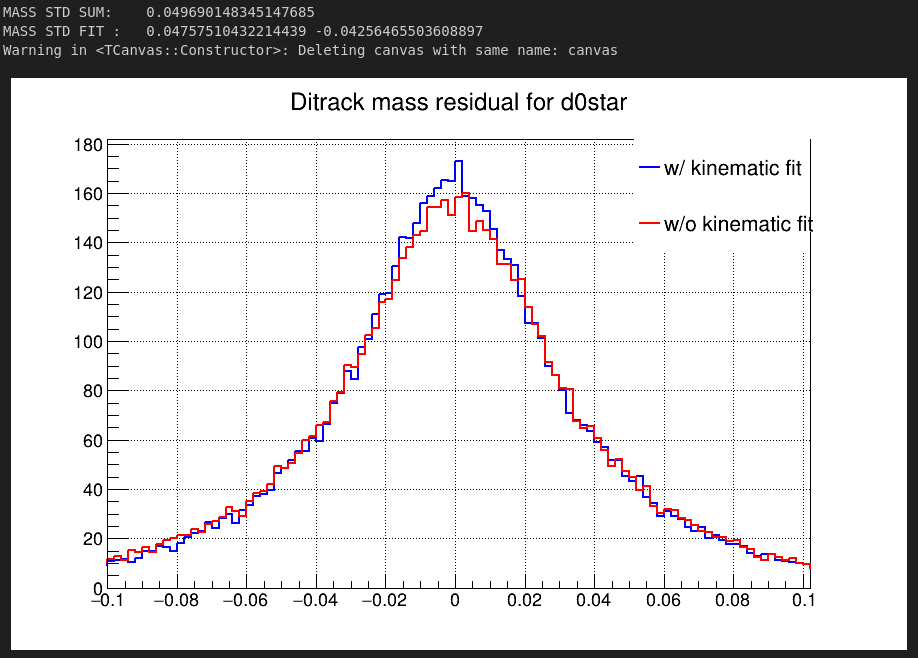
\includegraphics[width=0.45\mylength]{resources/plots/kinematic_fit_residual_d0star.png}
                \caption{\footnotesize (c)}
        \end{subfigure}%\begin{subfigure}[t]{0.50\mylength}
        \begin{subfigure}[t]{0.50\mylength}
                \centering
                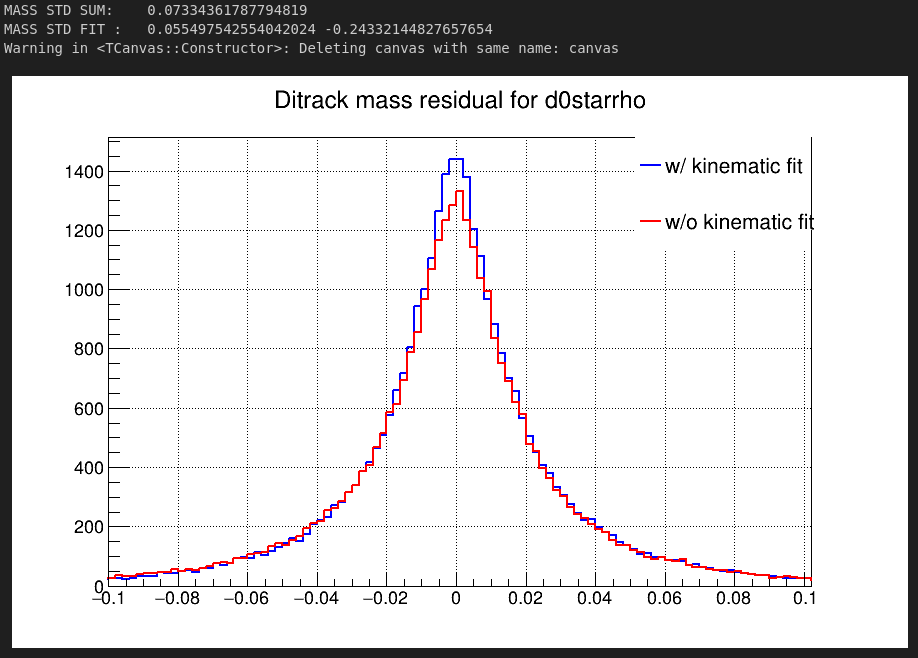
\includegraphics[width=0.45\mylength]{resources/plots/kinematic_fit_residual_d0starrho.png}
                \caption{\footnotesize (d)}
        \end{subfigure}%
        \vspace*{-0.0cm}
        \caption{Ditrack mass residuals for the different decay channels. (a) is for $\phi$, (b) is for $\omega$, (c) is for $D^{*0}$ 2-body and (d) is for $D^{*0}$ 3-body.}
        \label{fig:kinematic_fit_residuals}
        \vspace*{-0.0cm}
    \end{figure}
    Table \ref{tab:kinematic_fit_MSE} shows the mean squared errors with respect to generation-level, both with and without the kinematic fit for each channel. Applying the kinematic fit improves the reconstructed ditrack invariant mass values for all channels.

    \begin{table}[!ht]
        \centering
        
        \begin{tabular}{|l|c|C{2.9cm}@{}c|}
            \hline
            \cellcolor{lightgray}Decay channel & \cellcolor{lightgray}MSE without kinematic fit & \multicolumn{2}{c|}{\cellcolor{lightgray}MSE with kinematic fit} \\ \hline
            $\phi$          &37.8 MeV   &34.0 MeV  & (-10\%)   \\
            \r$\omega$        &\r ?? MeV   & .\r ?? MeV &\r (-x\%)  \\
            $D^{*0}$ 2-body &49.7 MeV   &47.6 MeV  & (-4\%)     \\
            $D^{*0}$ 3-body &73.3 MeV   &55.5 MeV  & (-24\%)    \\
            \hline
            \end{tabular}
        \caption{Mean squared errors (MSE) with and without the kinematic fit for each decay mode.}
        \label{tab:kinematic_fit_MSE}
    \end{table}
    
    \item[Meson mass hypothesis:] The simplest way to reconstruct the four-momentum of the full meson is to sum the four-momenta of the ditrack system and those from the photons compatible with the decay of neutral particles. This approach was initially used forall channels. Nevertheless, for the $\phi$, $\omega$ and $D^{*0}$ 3-body decay channels, additional corrections were applied.
    
    If we consider that the photons in the $\Delta R$ cone come from the $\pi^{0}\decaysto\gamma\gamma$ decay, when only one photon is recovered means that either both photons ended up in the same ECAL crystal, or that one of them was too soft to be measured ($\pT < 5\ \GeV$). Following the first hypothesis, we can interpret the energy deposited in the same ECAL cell as the energy from the full pion. To account for this, whenever we
    
    \todo{explain invariant meson mass correction with photons}

    \item[Meson transverse momentum correction:] \todo{explain regression BDT, long}

\end{myitemlist}

Tables \ref{tab:meson_selection_1} and \ref{tab:meson_selection_2} summarize the meson candidate selection criteria used.

\begin{table}[!ht]
    \centering
    \begin{tabular}{|l|c|c|}
        \hline
        \cellcolor{lightgray}Variable & \cellcolor{lightgray}$\phi(\pi^{\pm}\pi^{\mp}\pi^{0})$ & \cellcolor{lightgray}$\omega(\pi^{\pm}\pi^{\mp}\pi^{0})$ \\ \hline
        Meson mass                                              &$0.96\pm0.26$ GeV  &$0.785\pm0.215$ GeV    \\
        Ditrack mass                                            &$0.59\pm0.25$ GeV  &$0.47\pm0.15$ GeV      \\
        $\pT^{\text{diTrk}}$                                  &$>10$ GeV          &$>15$ GeV              \\
        $\pT^{\text{leadTrk}}$                                &$>5$ GeV           &$>8$ GeV               \\
        $\#\gamma^{\text{diTrk}}$                               &$>0$               &$>0$                   \\
        $\Delta(\phi^{\text{diTrk}}, \phi^{\gamma_\text{H}})$   &$\pi\pm2.3$    &$\pi\pm2.3$        \\
        $\Delta(\eta^{\text{diTrk}}, \eta^{\gamma_\text{H}})$   &$0\pm1.9$          &$0\pm1.9$              \\
        Iso                                                     &$>0.95$            &$>0.95$                \\
        \hline
        \end{tabular}
    \caption{Selection criteria applied to the $\phi$ and $\omega$ mesons used in the analysis.}
    \label{tab:meson_selection_1}
\end{table}

\begin{table}[!ht]
    \centering
    \begin{tabular}{|l|c|c|}
        \hline
        \cellcolor{lightgray}Variable & \cellcolor{lightgray}$D^{*0}(K^{\mp}\pi^{\pm}{\scriptstyle(\pi^{0}/\gamma)})$ & \cellcolor{lightgray}$D^{*0}(K^{\mp}\pi^{\pm}\pi^{0}{\scriptstyle(\pi^{0}/\gamma)})$ \\ \hline
        Meson mass                                              &                   &\r $x.xx\pm x.xx$ GeV  \\
        Ditrack mass                                            &$1.865\pm0.060$ GeV&\r $x.xx\pm x.xx$ GeV  \\
        $\pT^{\text{diTrk}}$                                  &$>40$ GeV          &\r $>xx$ GeV           \\
        $\pT^{\text{leadTrk}}$                                &$>21$ GeV          &\r $>xx$ GeV           \\
        $\#\gamma^{\text{diTrk}}$                               &                   &\r $>xx$               \\
        $\Delta(\phi^{\text{diTrk}}, \phi^{\gamma_\text{H}})$   &$\pi\pm2.3$    &\r $\pi\pm2.3$     \\
        $\Delta(\eta^{\text{diTrk}}, \eta^{\gamma_\text{H}})$   &$0\pm1.9$          &\r $0\pm1.9$           \\
        Iso                                                     &$>0.91$            &\r $>  xx$             \\
        \hline
        \end{tabular}
    \caption{Selection criteria applied to each channel of the $D^{*0}$ meson decay used in the analysis.}
    \label{tab:meson_selection_2}
\end{table}

\todo{Talk about the criteria used a bit}

%\section{Corrections to data and simulations}\label{sec:corrections}

%\todo{Pileup reweighting, L1 prefiring corrections, photon scale and resolution, photon mvaid efficiency, Lepton ID reconstruction efficiency and energy scale (?), meson reconstruction, triggers scale factors}

\section{Event selection}\label{sec:event_selection}

\todo{Gluon fusion selection for each channel}

\todo{Explain we only pick one goodphoton/goodmeson for each event, and criteria}

\section{Signal and background modelling}\label{sec:modelling}

\todo{signal, background model from MC and data, bias studies}

\section{Results}\label{sec:results}

\todo{Present results}

\section{Future potential improvements}\label{sec:future_improvements}

\todo{talk about MVA, data-MC corrections, and what are next steps before unblinding data}

